\documentclass[8pt]{beamer}
\usepackage[slovene]{babel}
\usepackage[utf8]{inputenc}
\usepackage[T1]{fontenc}
\usepackage{lmodern}
\usepackage{mathptmx}
\usepackage{helvet}
\usepackage{courier}
\usepackage{hyperref}
\usepackage{tikz}
\usepackage{enumerate}
\setbeamertemplate{caption}[numbered]

\usetheme{CambridgeUS}

\setbeamercolor*{item}{fg=red}
\setbeamercolor*{label}{fg=red}

\begin{document}


\title[Reševanje TSP s k-opt in LK algoritmom]{Reševanje problema trgovskega potnika s k-optimalnim in
Lin-Kernighanovim algoritmom}
\author[Žan Jernejčič in Ines Šilc]{Žan Jernejčič in Ines Šilc}
\institute [FMF]{Fakulteta za matematiko in fiziko}

\begin{frame}
	\titlepage
\end {frame}

\section[Definiranje problema]{Definiranje problema}
\begin{frame}
\frametitle{Definicija problema}
Problem trgovskega potnika oziroma Travelling salesman problem (krajše TSP) je problem, kjer imamo podanih $n$ mest in razdalje med vsemi (za vsak par mest imamo torej podano, koliko sta si oddaljeni). Zanima nas, ali lahko obiščemo vsako mesto in se na koncu vrnemo v prvotno mesto. Če označimo $d_{i, j}$ kot razdaljo mad $i$-tim in $j$-tim mestom, iščemo torej:\\

$$
\min_{\pi \in S_n} \sum\limits_{i=1}^{n-1} d_{\pi (i), \pi (i+1)} + d_{\pi (n), \pi (1)}
$$

 kjer je $S_n$ množica vseh permutacij danih $n$ mest. \\
\vspace{5mm}
Naivna rešitev je očitna, pogledamo $(n-1)!$ kombinacij, torej iz vsakega mesta v vsako drugo mesto, si zapišemo vse kombinacije in kakšno razdaljo smo prepotovali, ter izberemo tisto možnost, kjer je bila razdalja najkrajša.\\ 
\end{frame}

\begin{frame}
\frametitle{Programsko okolje}
Za projekt sva uporabila programski jezik \texttt{python}. Uporabljala sva naslednje pakete:

\begin{itemize}
\setlength\itemsep{1em}
\item \texttt{networkx}: za definiranje in generiranje grafov

\item \texttt{random}: za generiranje naključnih števil in seznamov

\item \texttt{matplotlib}: za izrisovanje grafov

\item \texttt{time}: za mertive časovne zahtevnosti

\item \texttt{itertools}: za generiranje prvotne permutacije

\end{itemize}


Za preverjanje veljavnosti poti v grafu za problem potujočega trgovca, morava vedeti:

\begin{itemize}
\setlength\itemsep{1em}
\item Vsaka pot trgovca bo morala imeti vsa vozlišča primarnega grafa
\item Vsaka pot trgovca bo morala imeti točno toliko povezav kot vozlišč
\item Dolžina poti bo morala biti enaka številu vozlišč -1
\end{itemize}
\end{frame}

\begin{frame}[fragile]
\frametitle{Osnovni algoritem}
\begin{verbatim}
def dva_opt(graf, pot):

    najboljsa_pot = pot
    cena = cena_poti(graf, pot)    
    
    izboljsanje = True
    while izboljsanje:
        izboljsanje = False
        for i in range(1,len(pot) - 2):
            for j in range(i + 1, len(pot)):
                if j - i == 1: continue
                nova_pot = pot[:]
                nova_pot[i:j] = pot[j - 1:i - 1:-1]
                nova_cena = cena_poti(graf, nova_pot)
                if nova_cena < cena:
                    najboljsa_pot = nova_pot[:]
                    cena = nova_cena
                    izboljsanje = True
        pot = najboljsa_pot
        
    return (pot)
\end{verbatim}
\end{frame}

\section[Primeri]{Primeri}
\begin{frame}
\frametitle{Primer grafa}
\begin{equation}
\label{matrika}
\begin{bmatrix} 
0&2&3&4&1000\\
2&0&8&9&10\\
3&8&0&14&15\\
4&9&14&0&20\\
1000&10&15&20&0\\
\end{bmatrix}
\end{equation}
\end{frame}

\begin{frame}
  \begin{figure}
  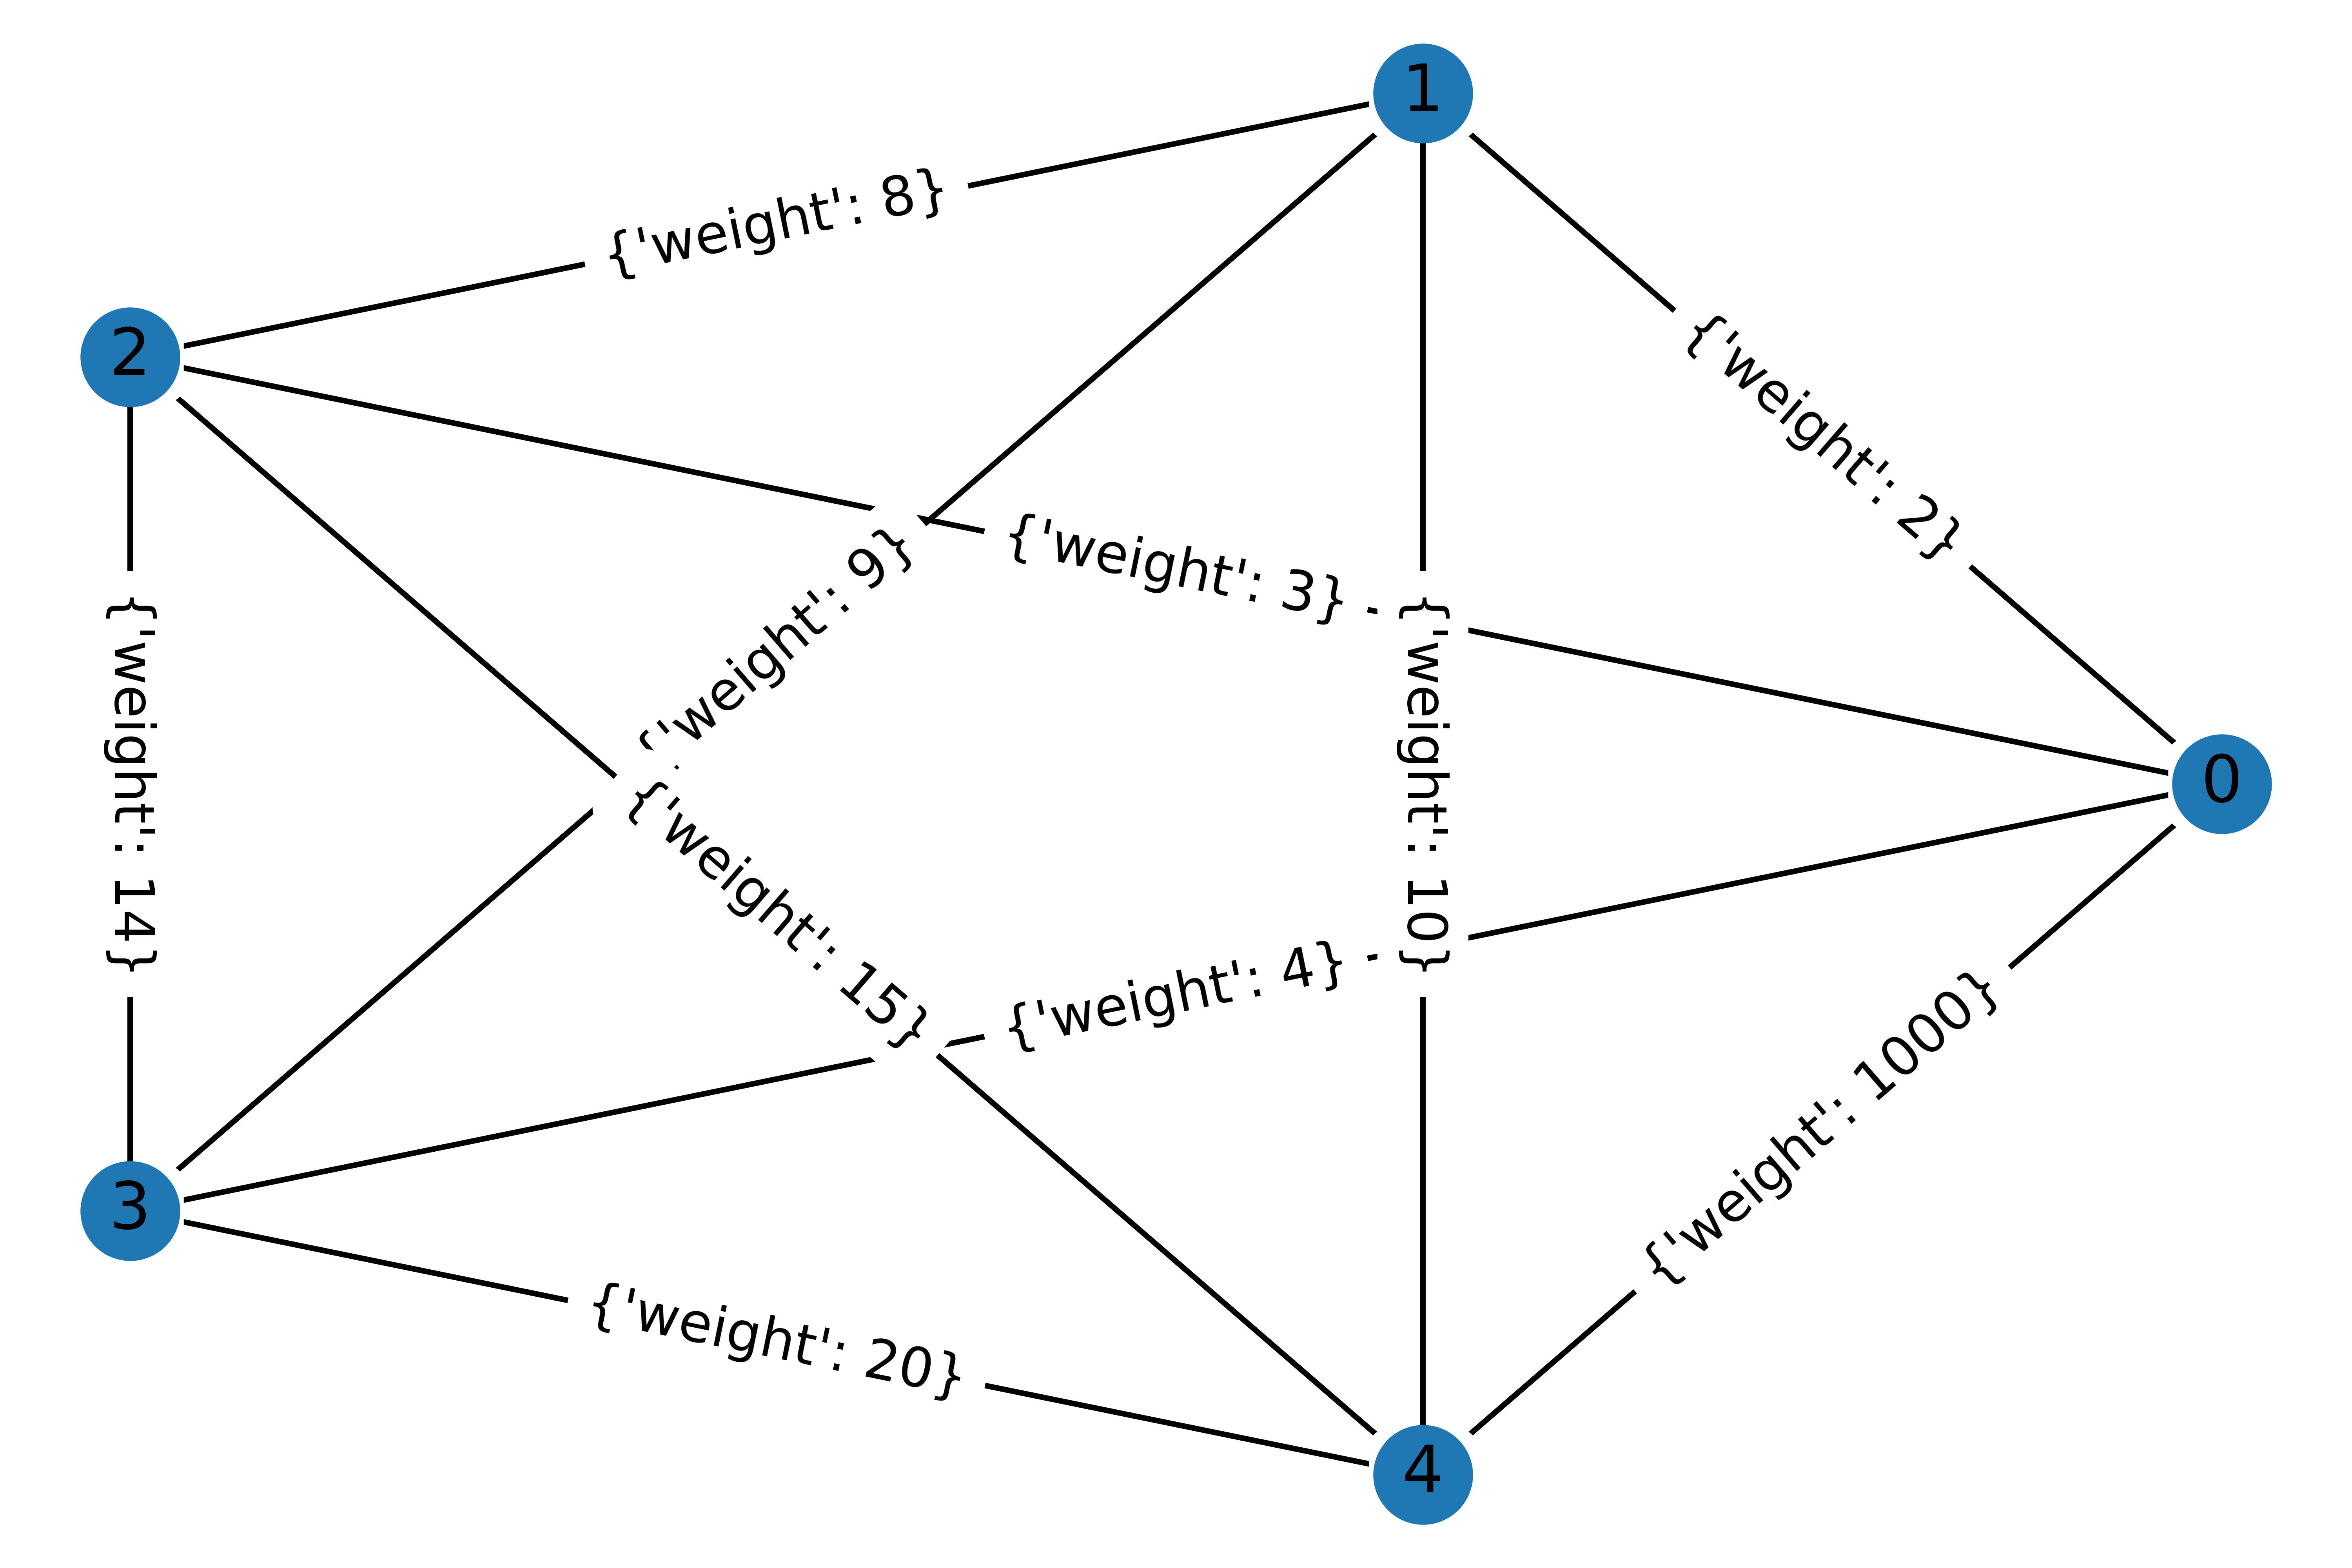
\includegraphics[width=10cm]{primeri/primer1.png}
 	\caption{Poln graf na 5 vozliščih}
	\label{Slika 1}
	\end{figure}
\end{frame}

\begin{frame}
\begin{figure}
  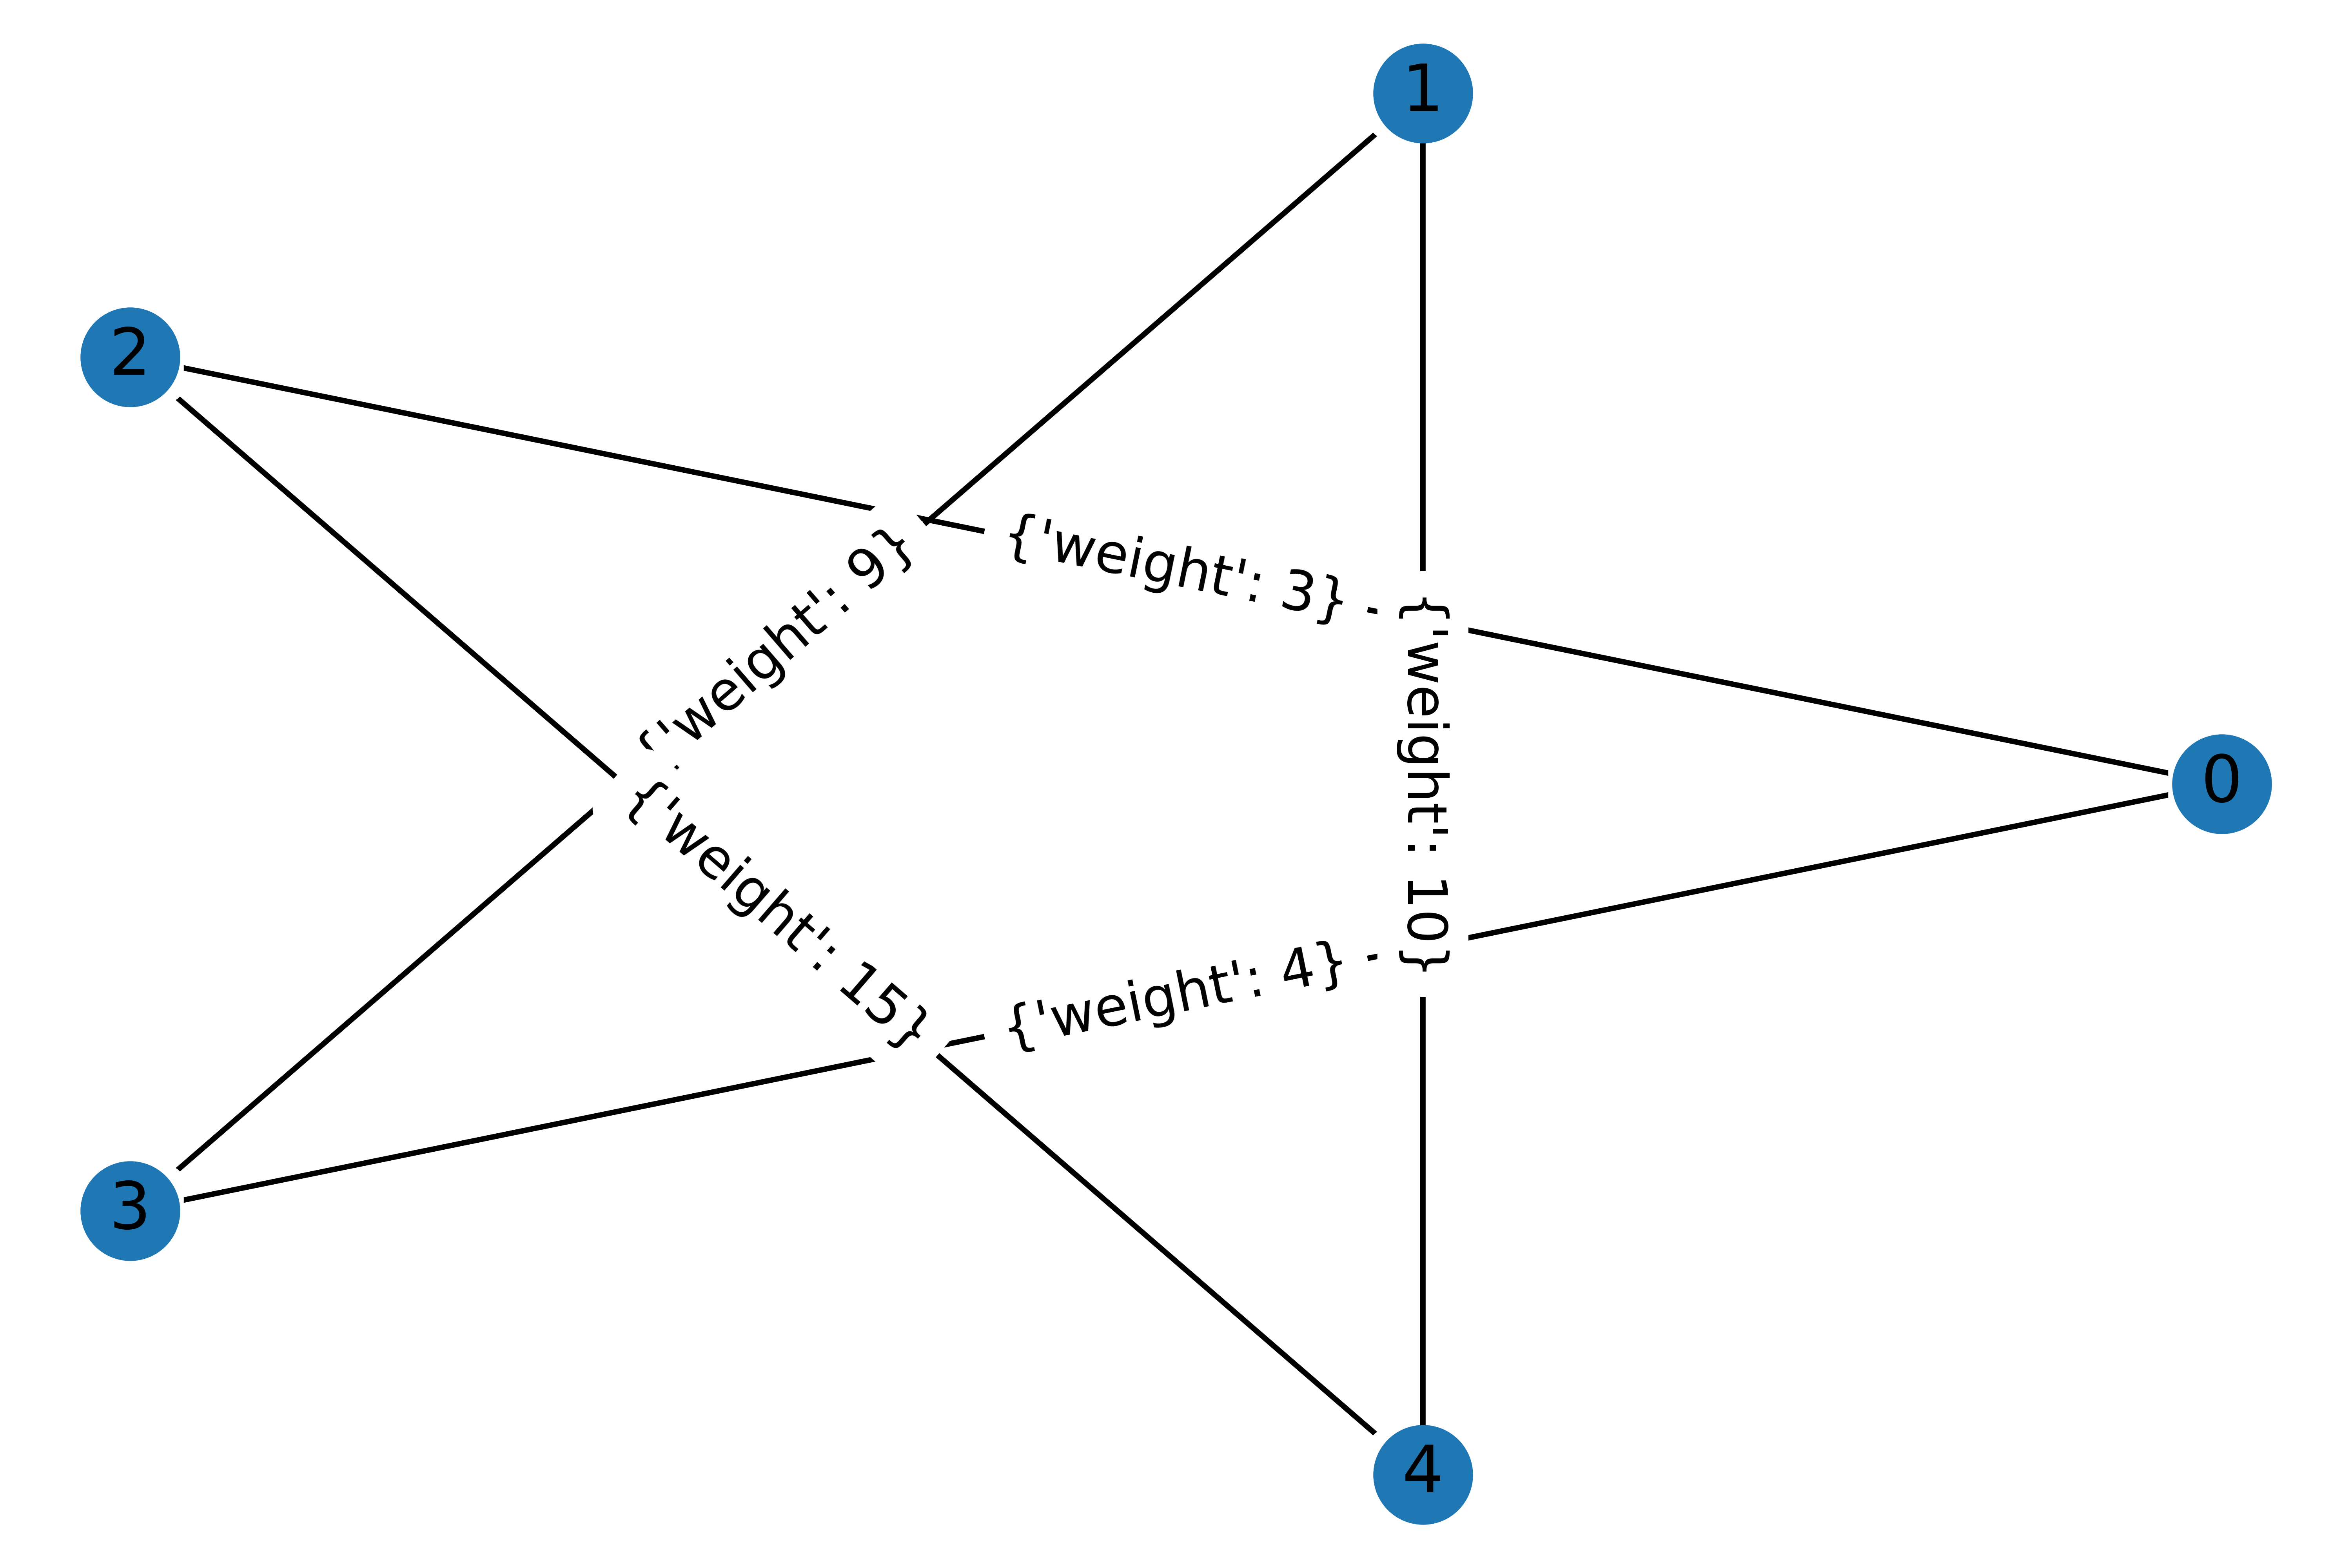
\includegraphics[width=10cm]{primeri/primer1_2opt.png}
\caption{2-opt}
\label{Slika 2}
\end{figure}
\end{frame}

\begin{frame}
  \begin{figure}
  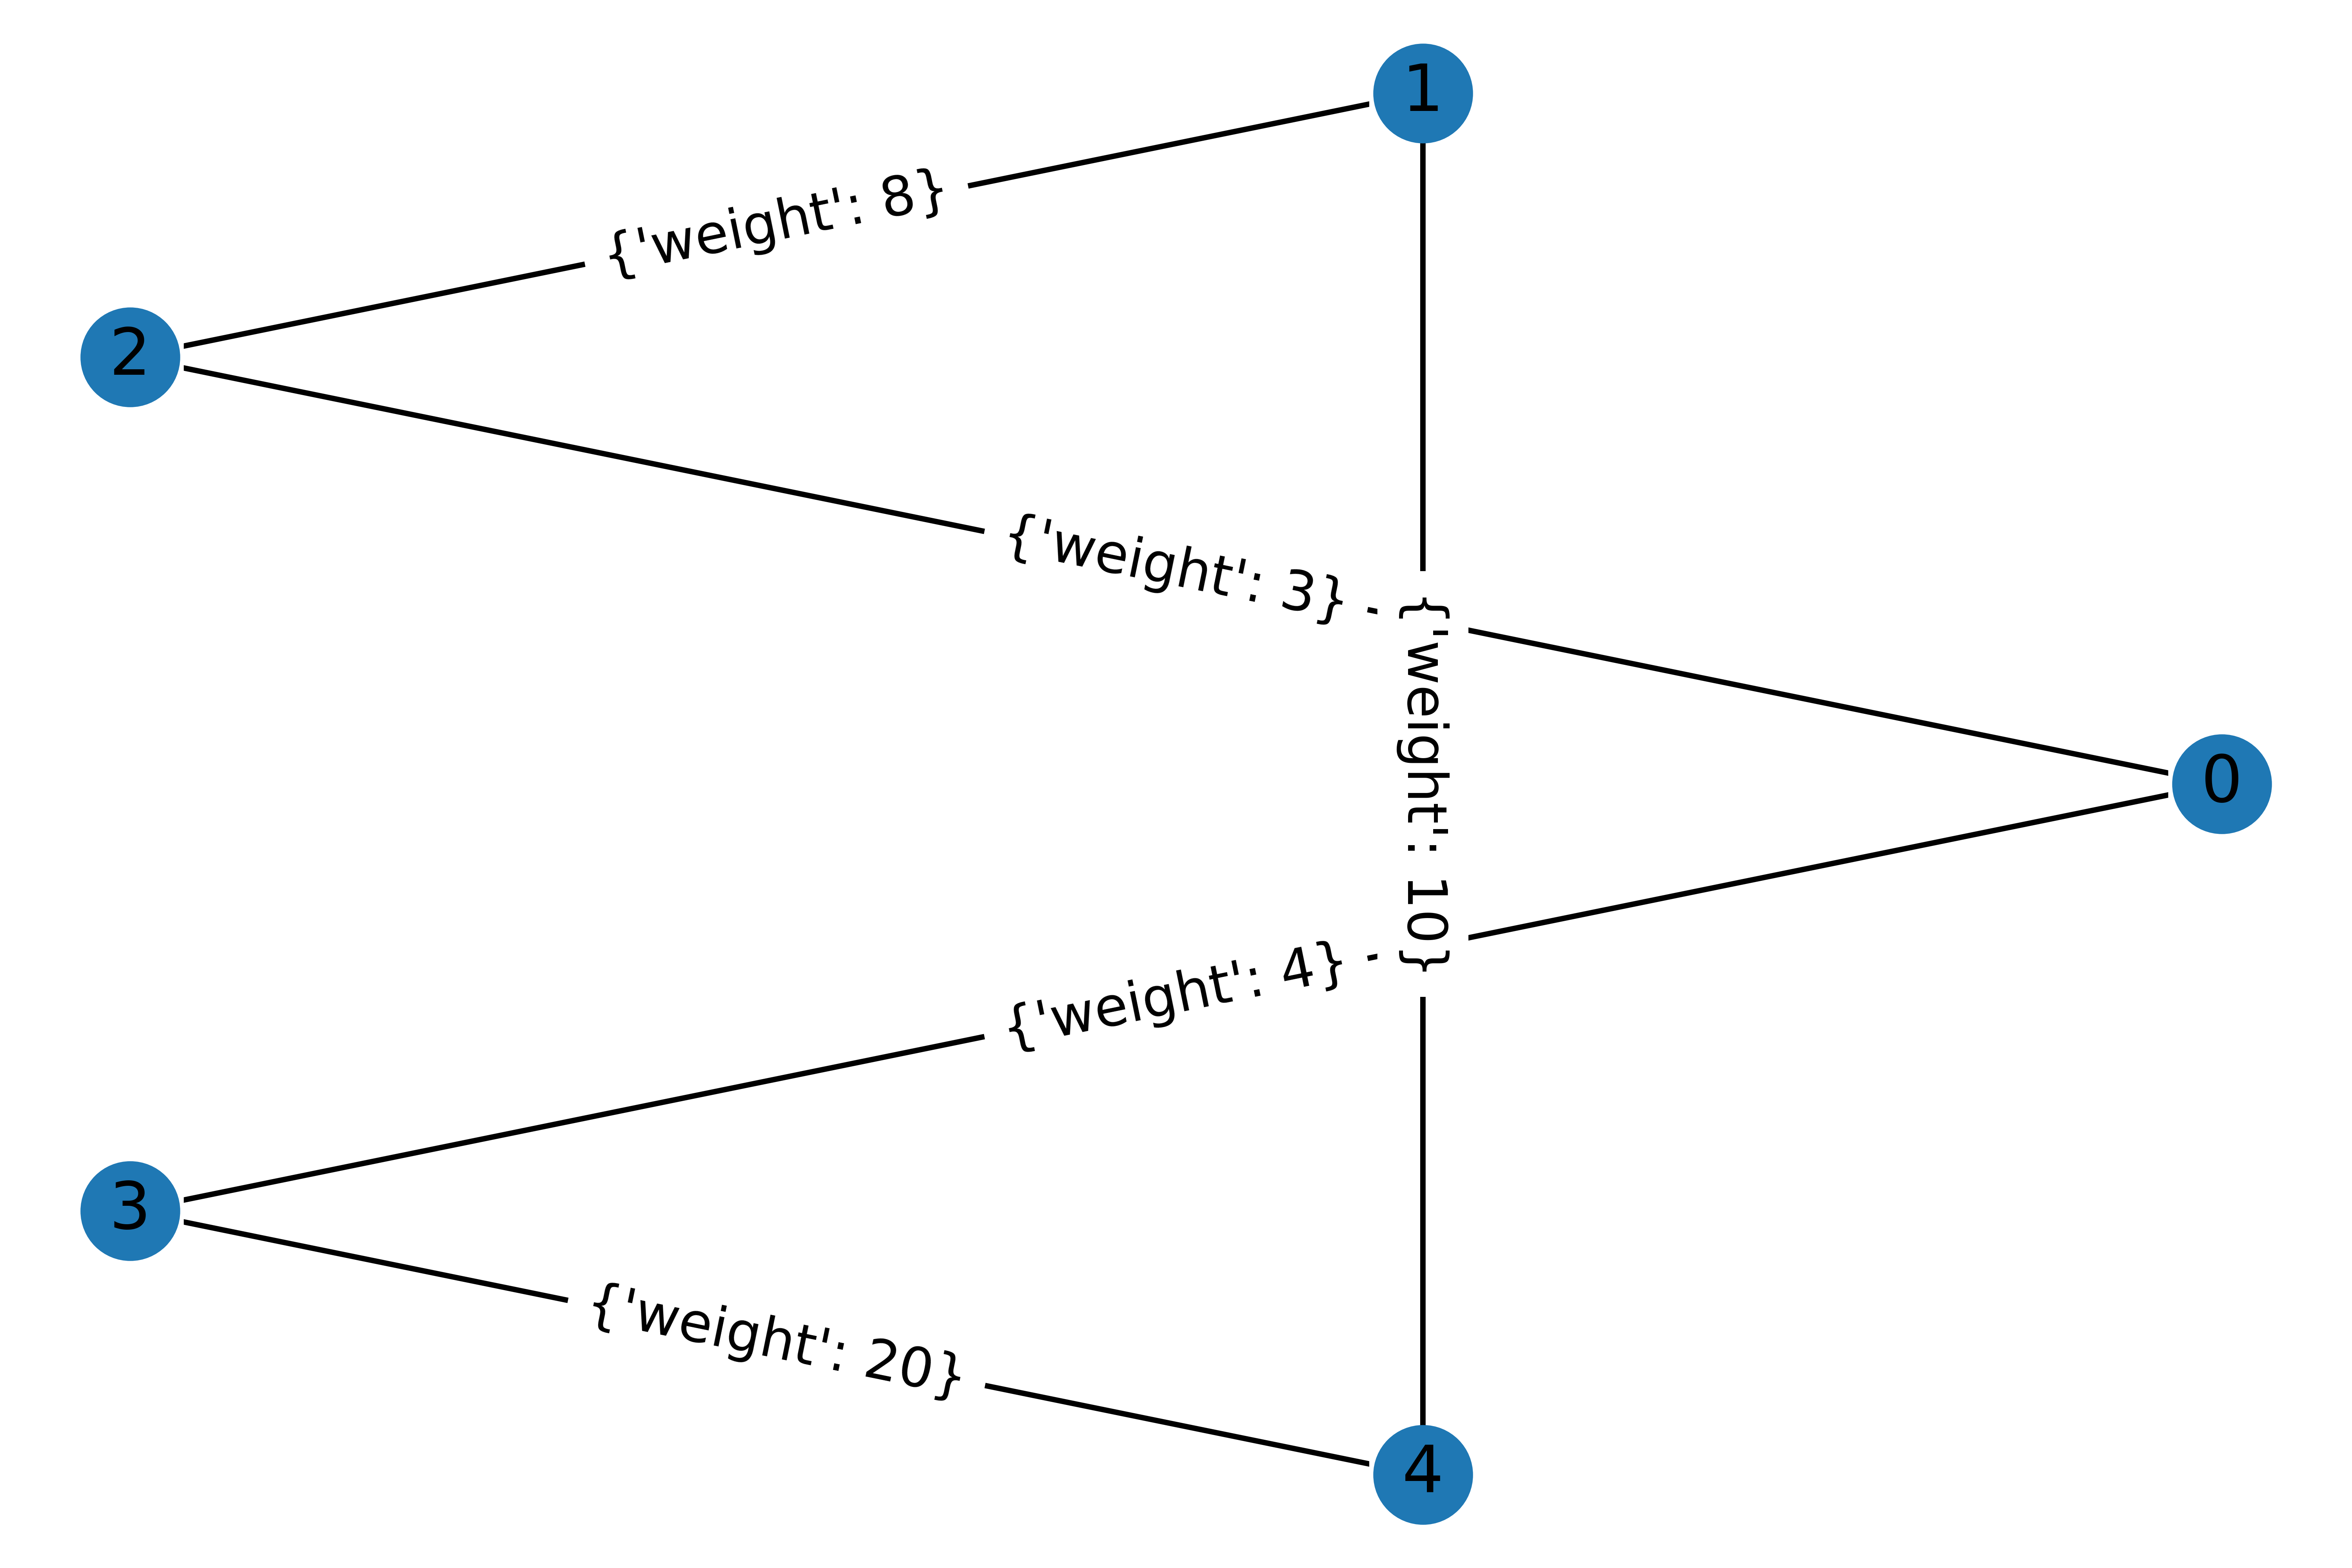
\includegraphics[width=10cm]{primeri/primer1_3opt.png}
 	\caption{3-opt}
	\label{Slika 3}
	\end{figure}
\end{frame}

\begin{frame}
\begin{figure}
  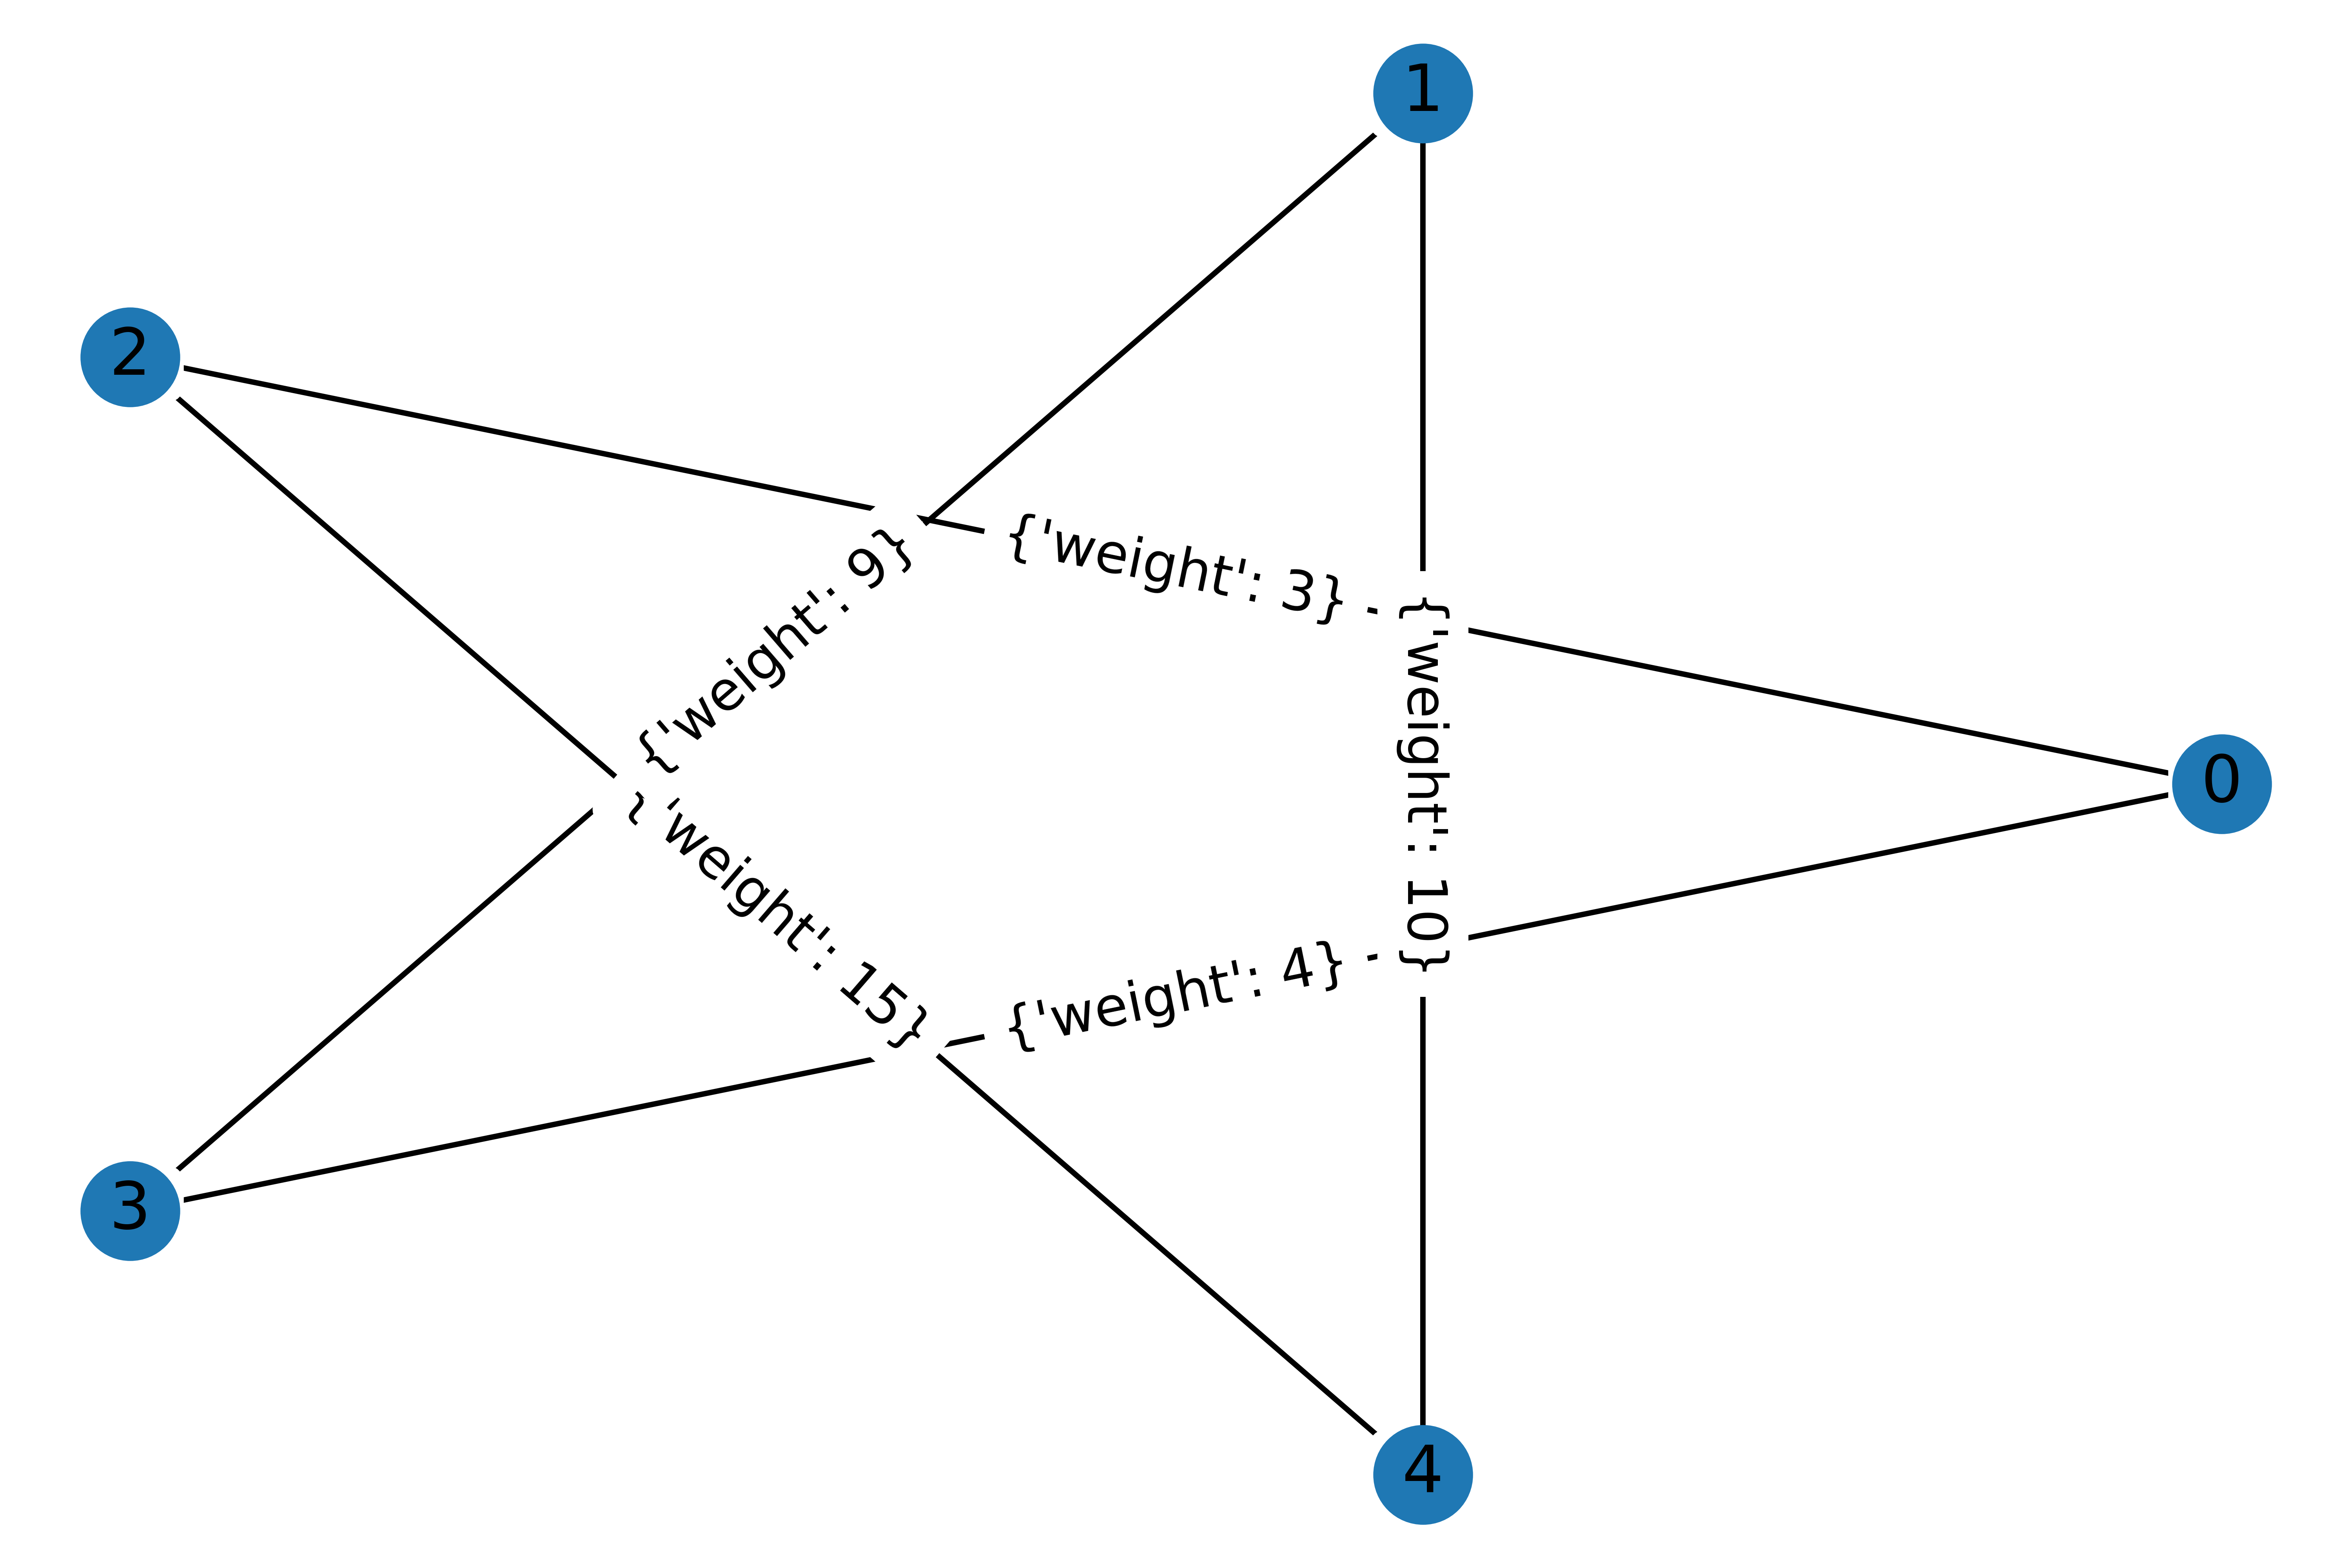
\includegraphics[width=10cm]{primeri/primer1_lk.png}
\caption{LK}
\label{Slika 4}
\end{figure}
\end{frame}

\begin{frame}
  \begin{figure}
  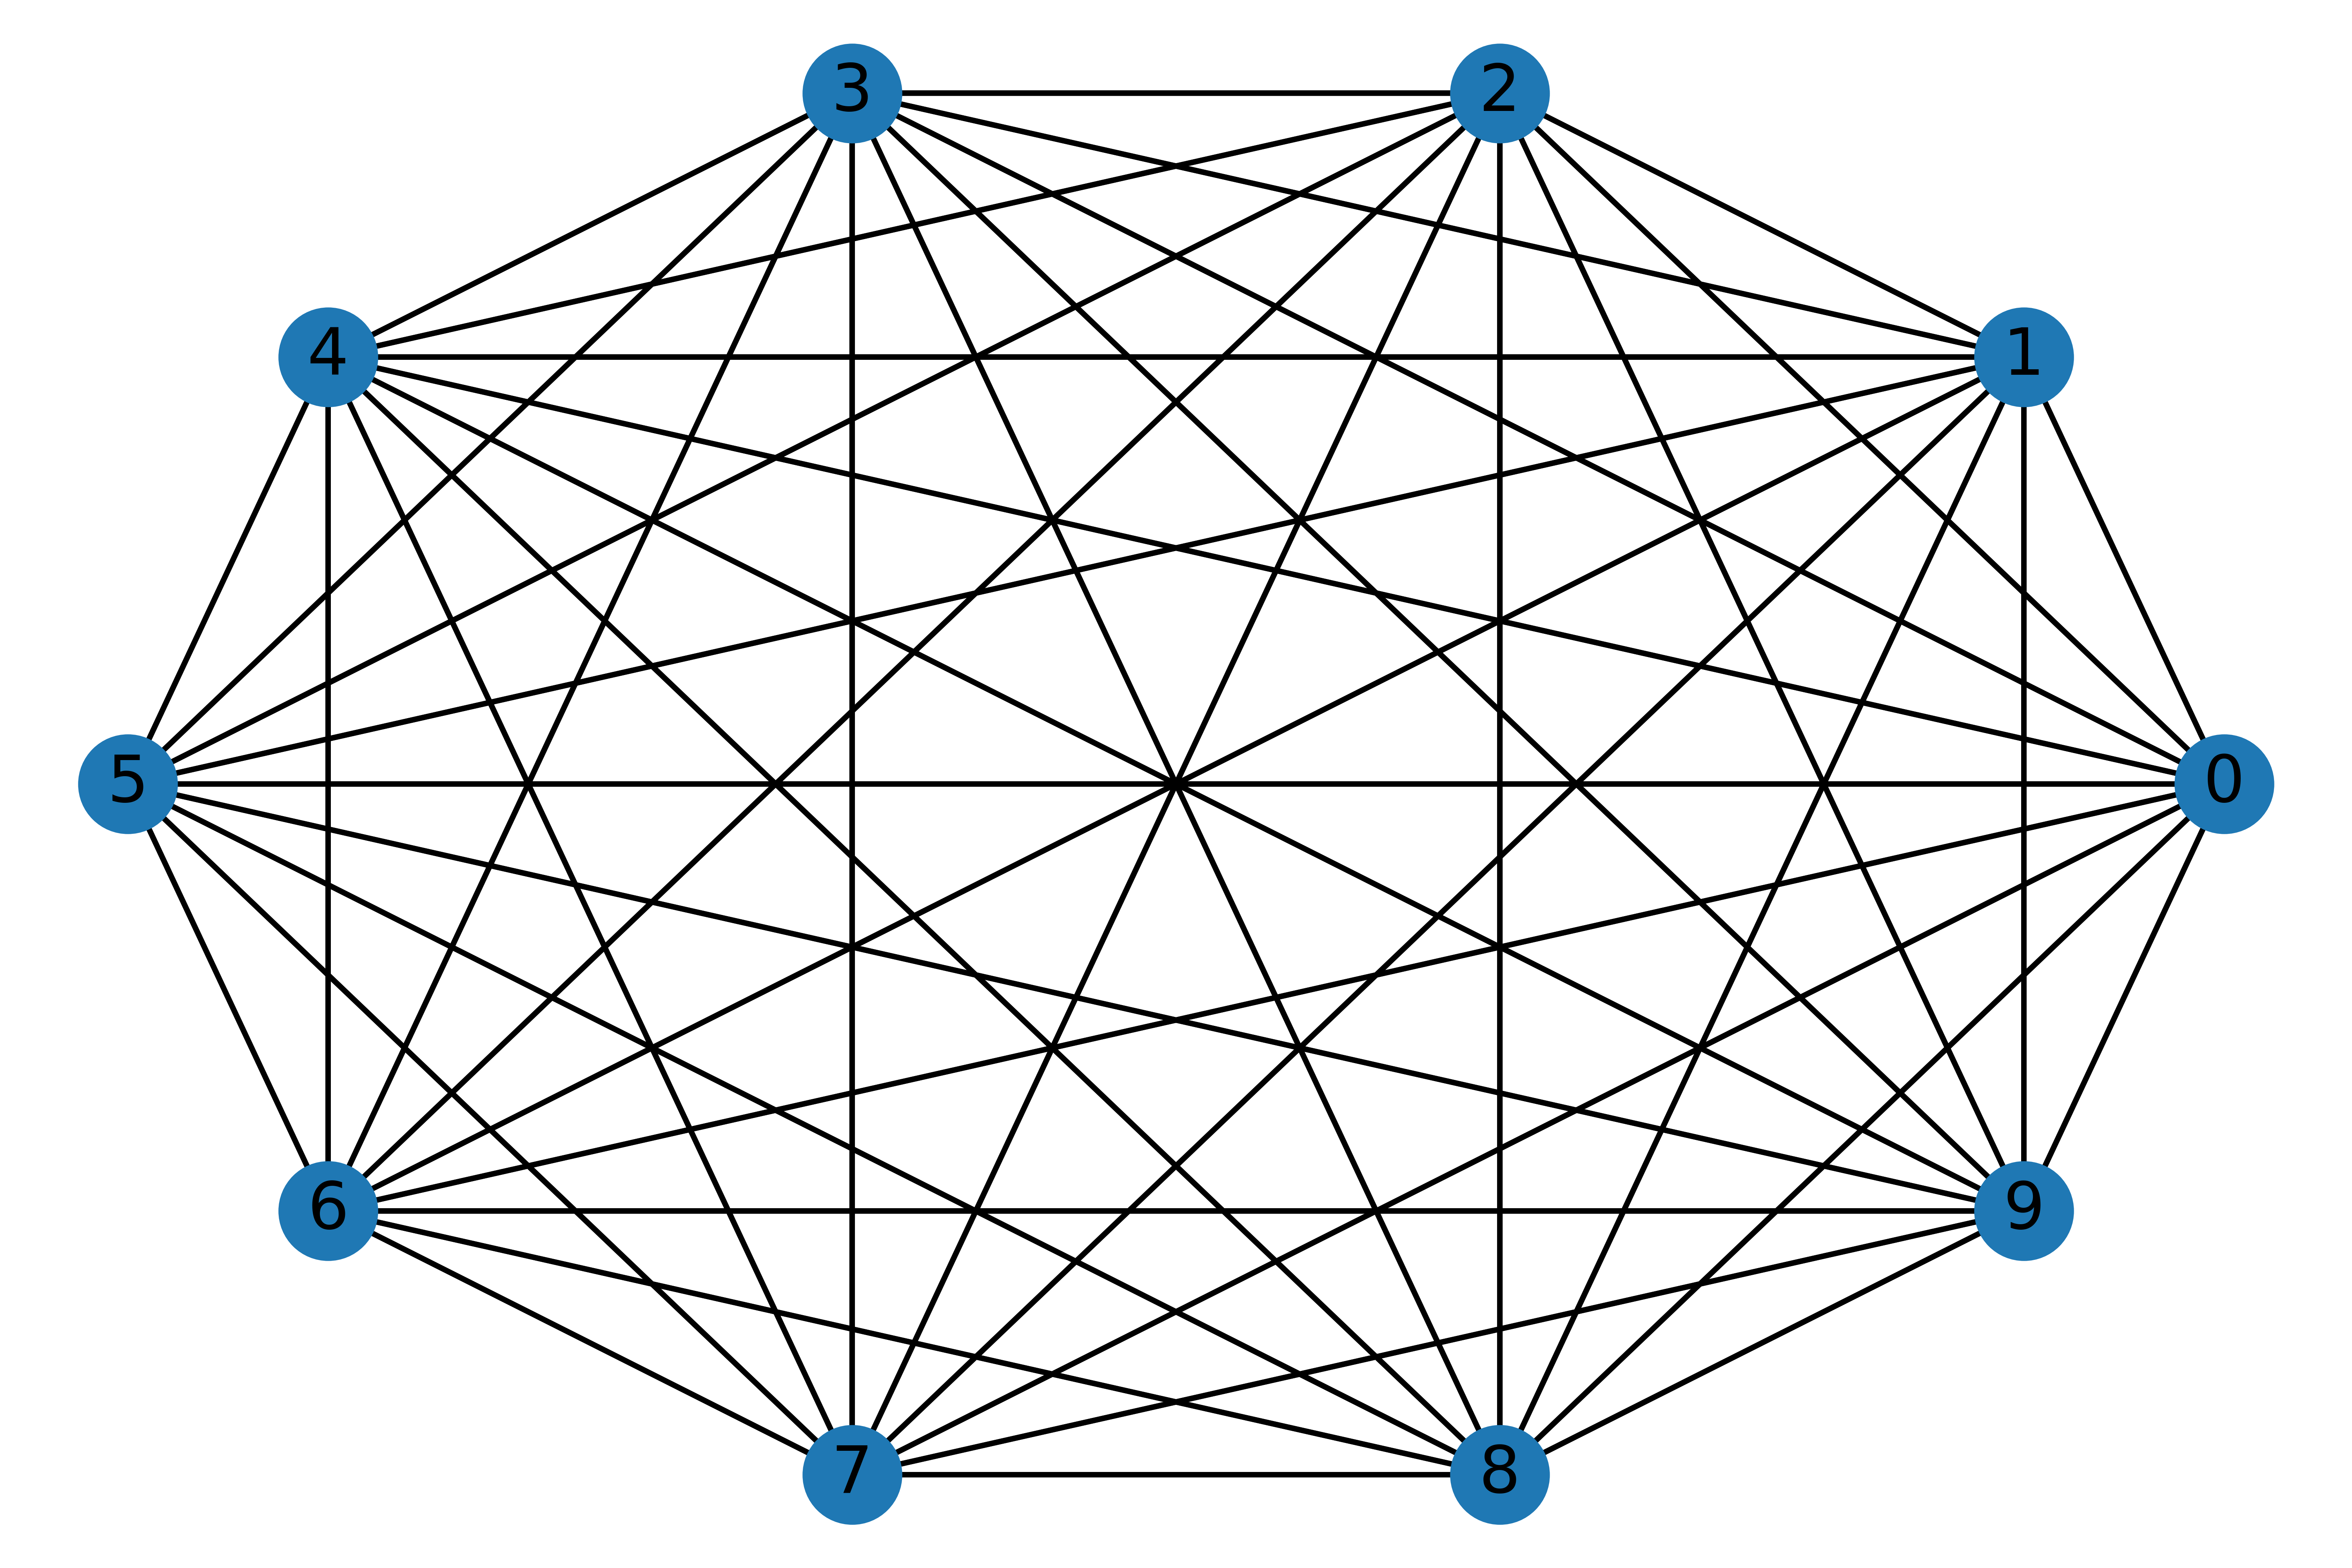
\includegraphics[width=10cm]{primeri/primer2.png}
 	\caption{Poln graf na 5 vozliščih}
	\label{Slika 5}
	\end{figure}
\end{frame}

\begin{frame}
\begin{figure}
  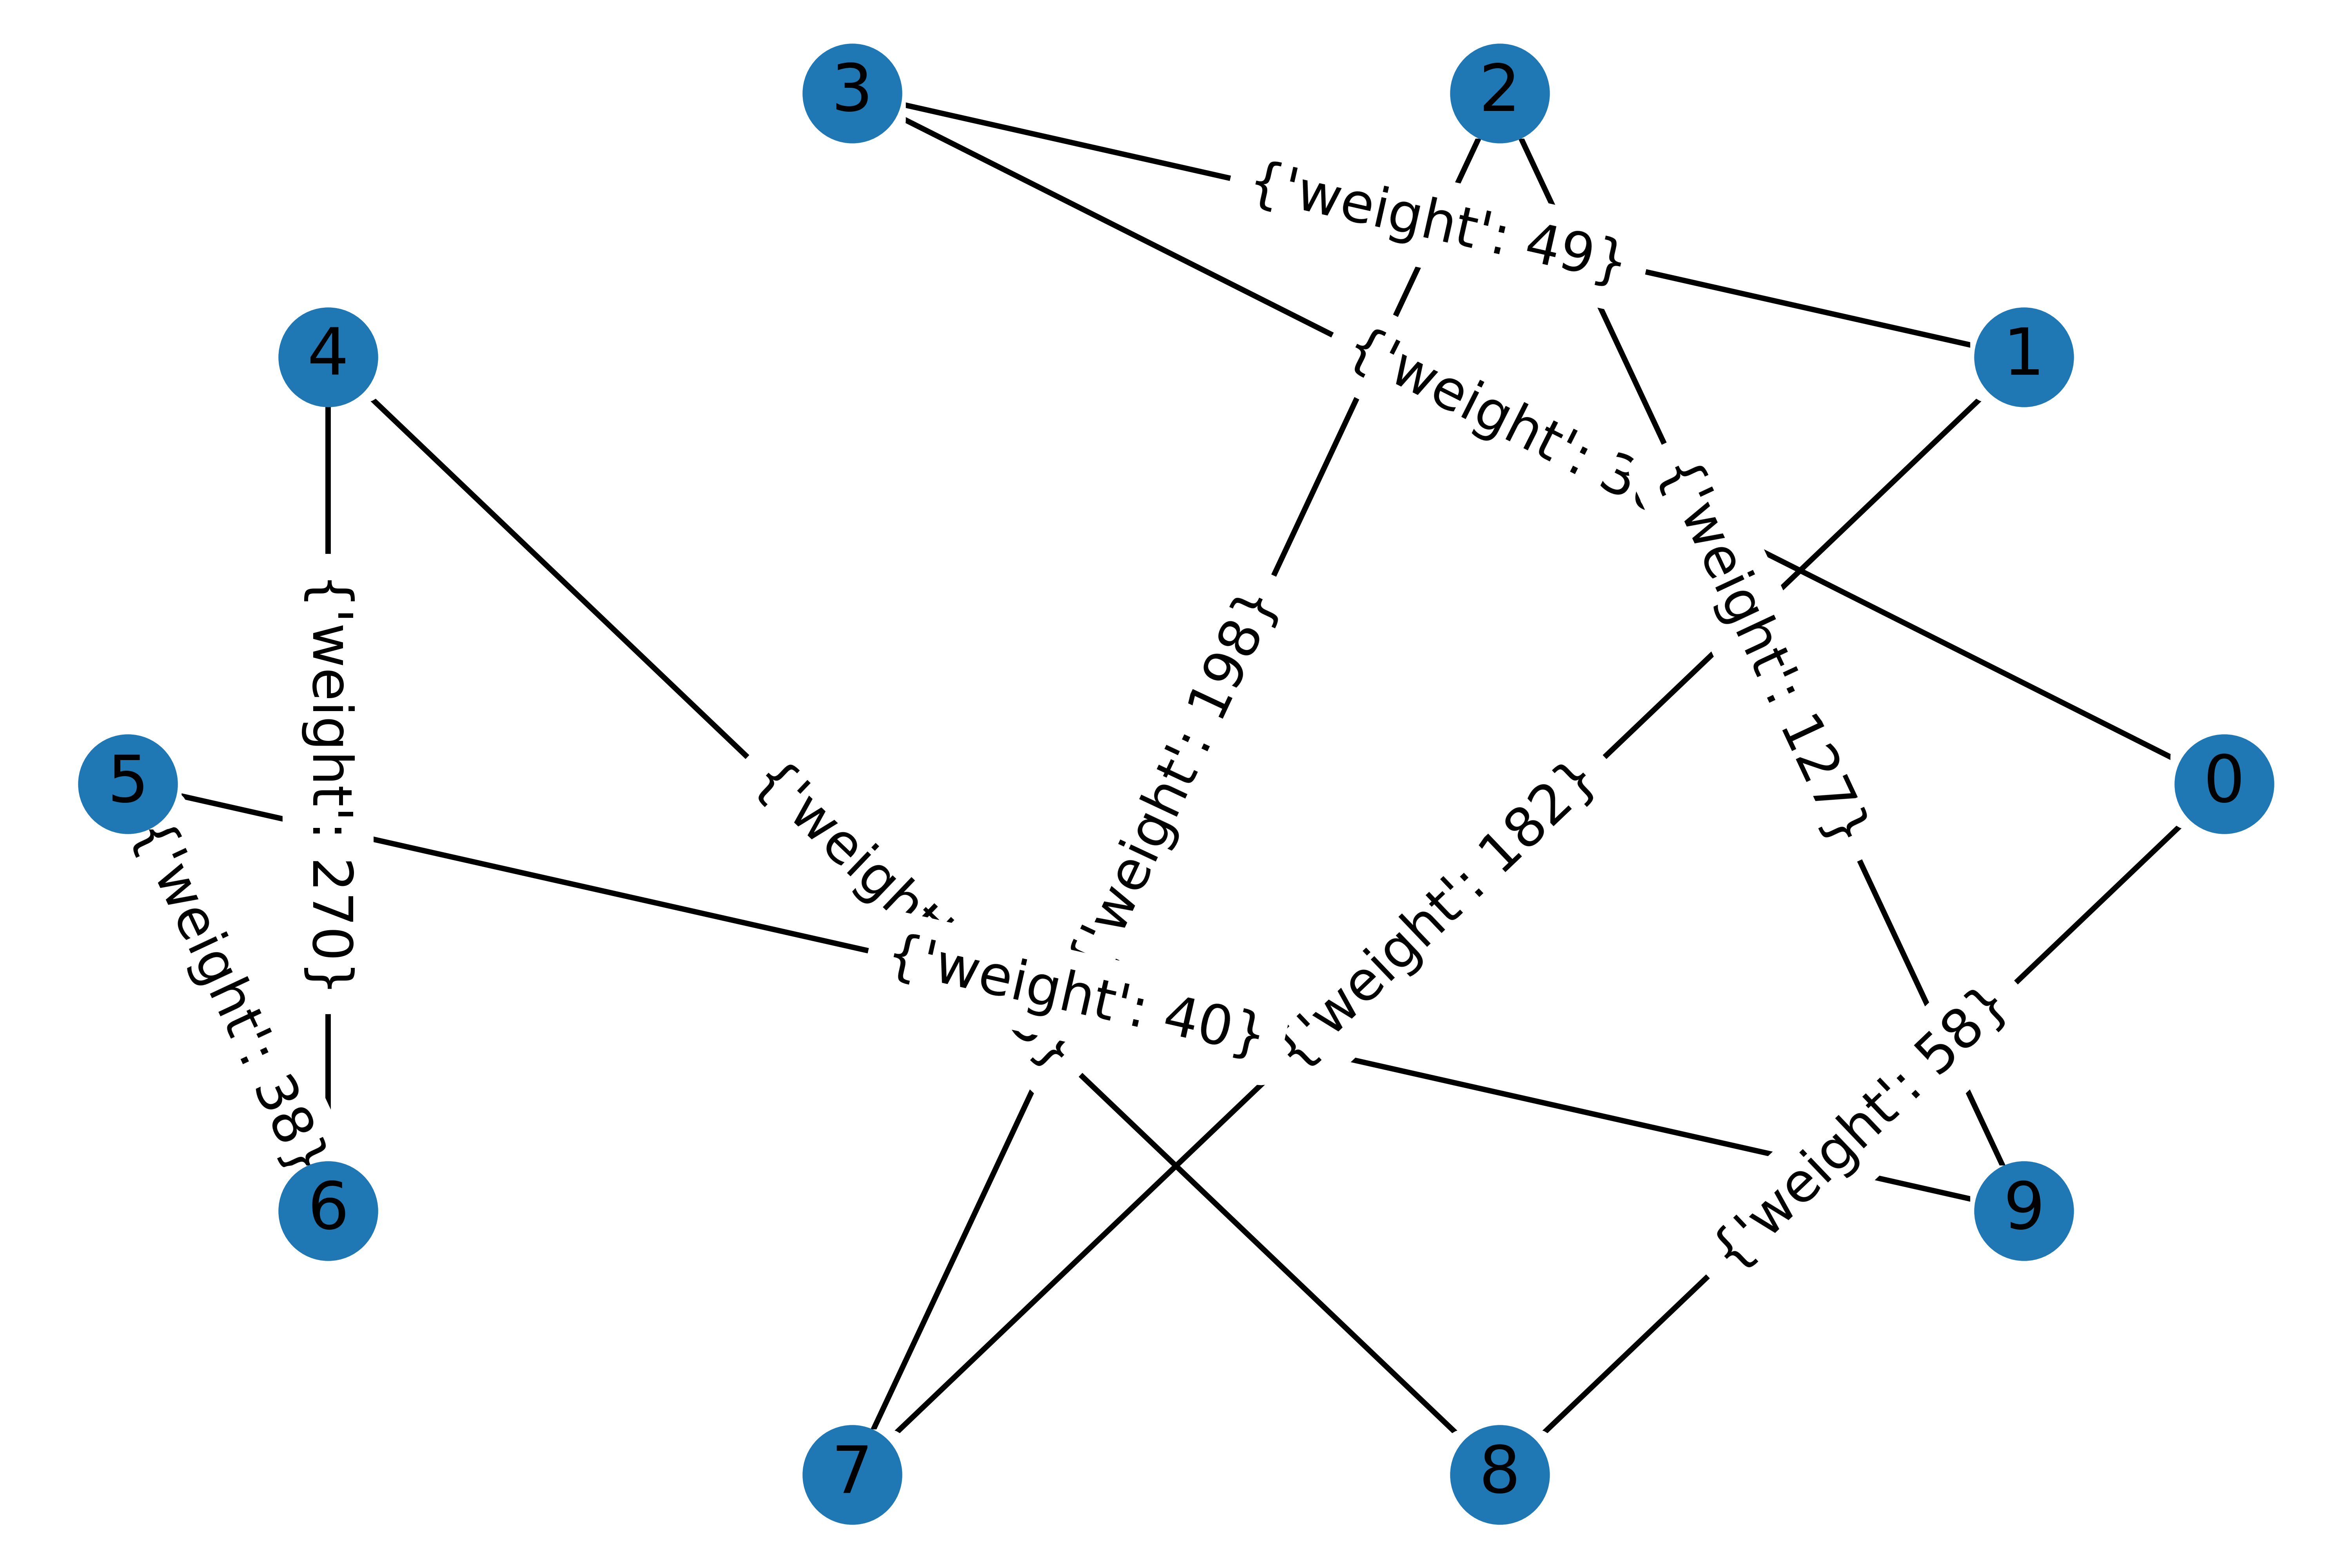
\includegraphics[width=10cm]{primeri/primer2_2opt.png}
\caption{2-opt}
\label{Slika 6}
\end{figure}
\end{frame}


\begin{frame}
  \begin{figure}
  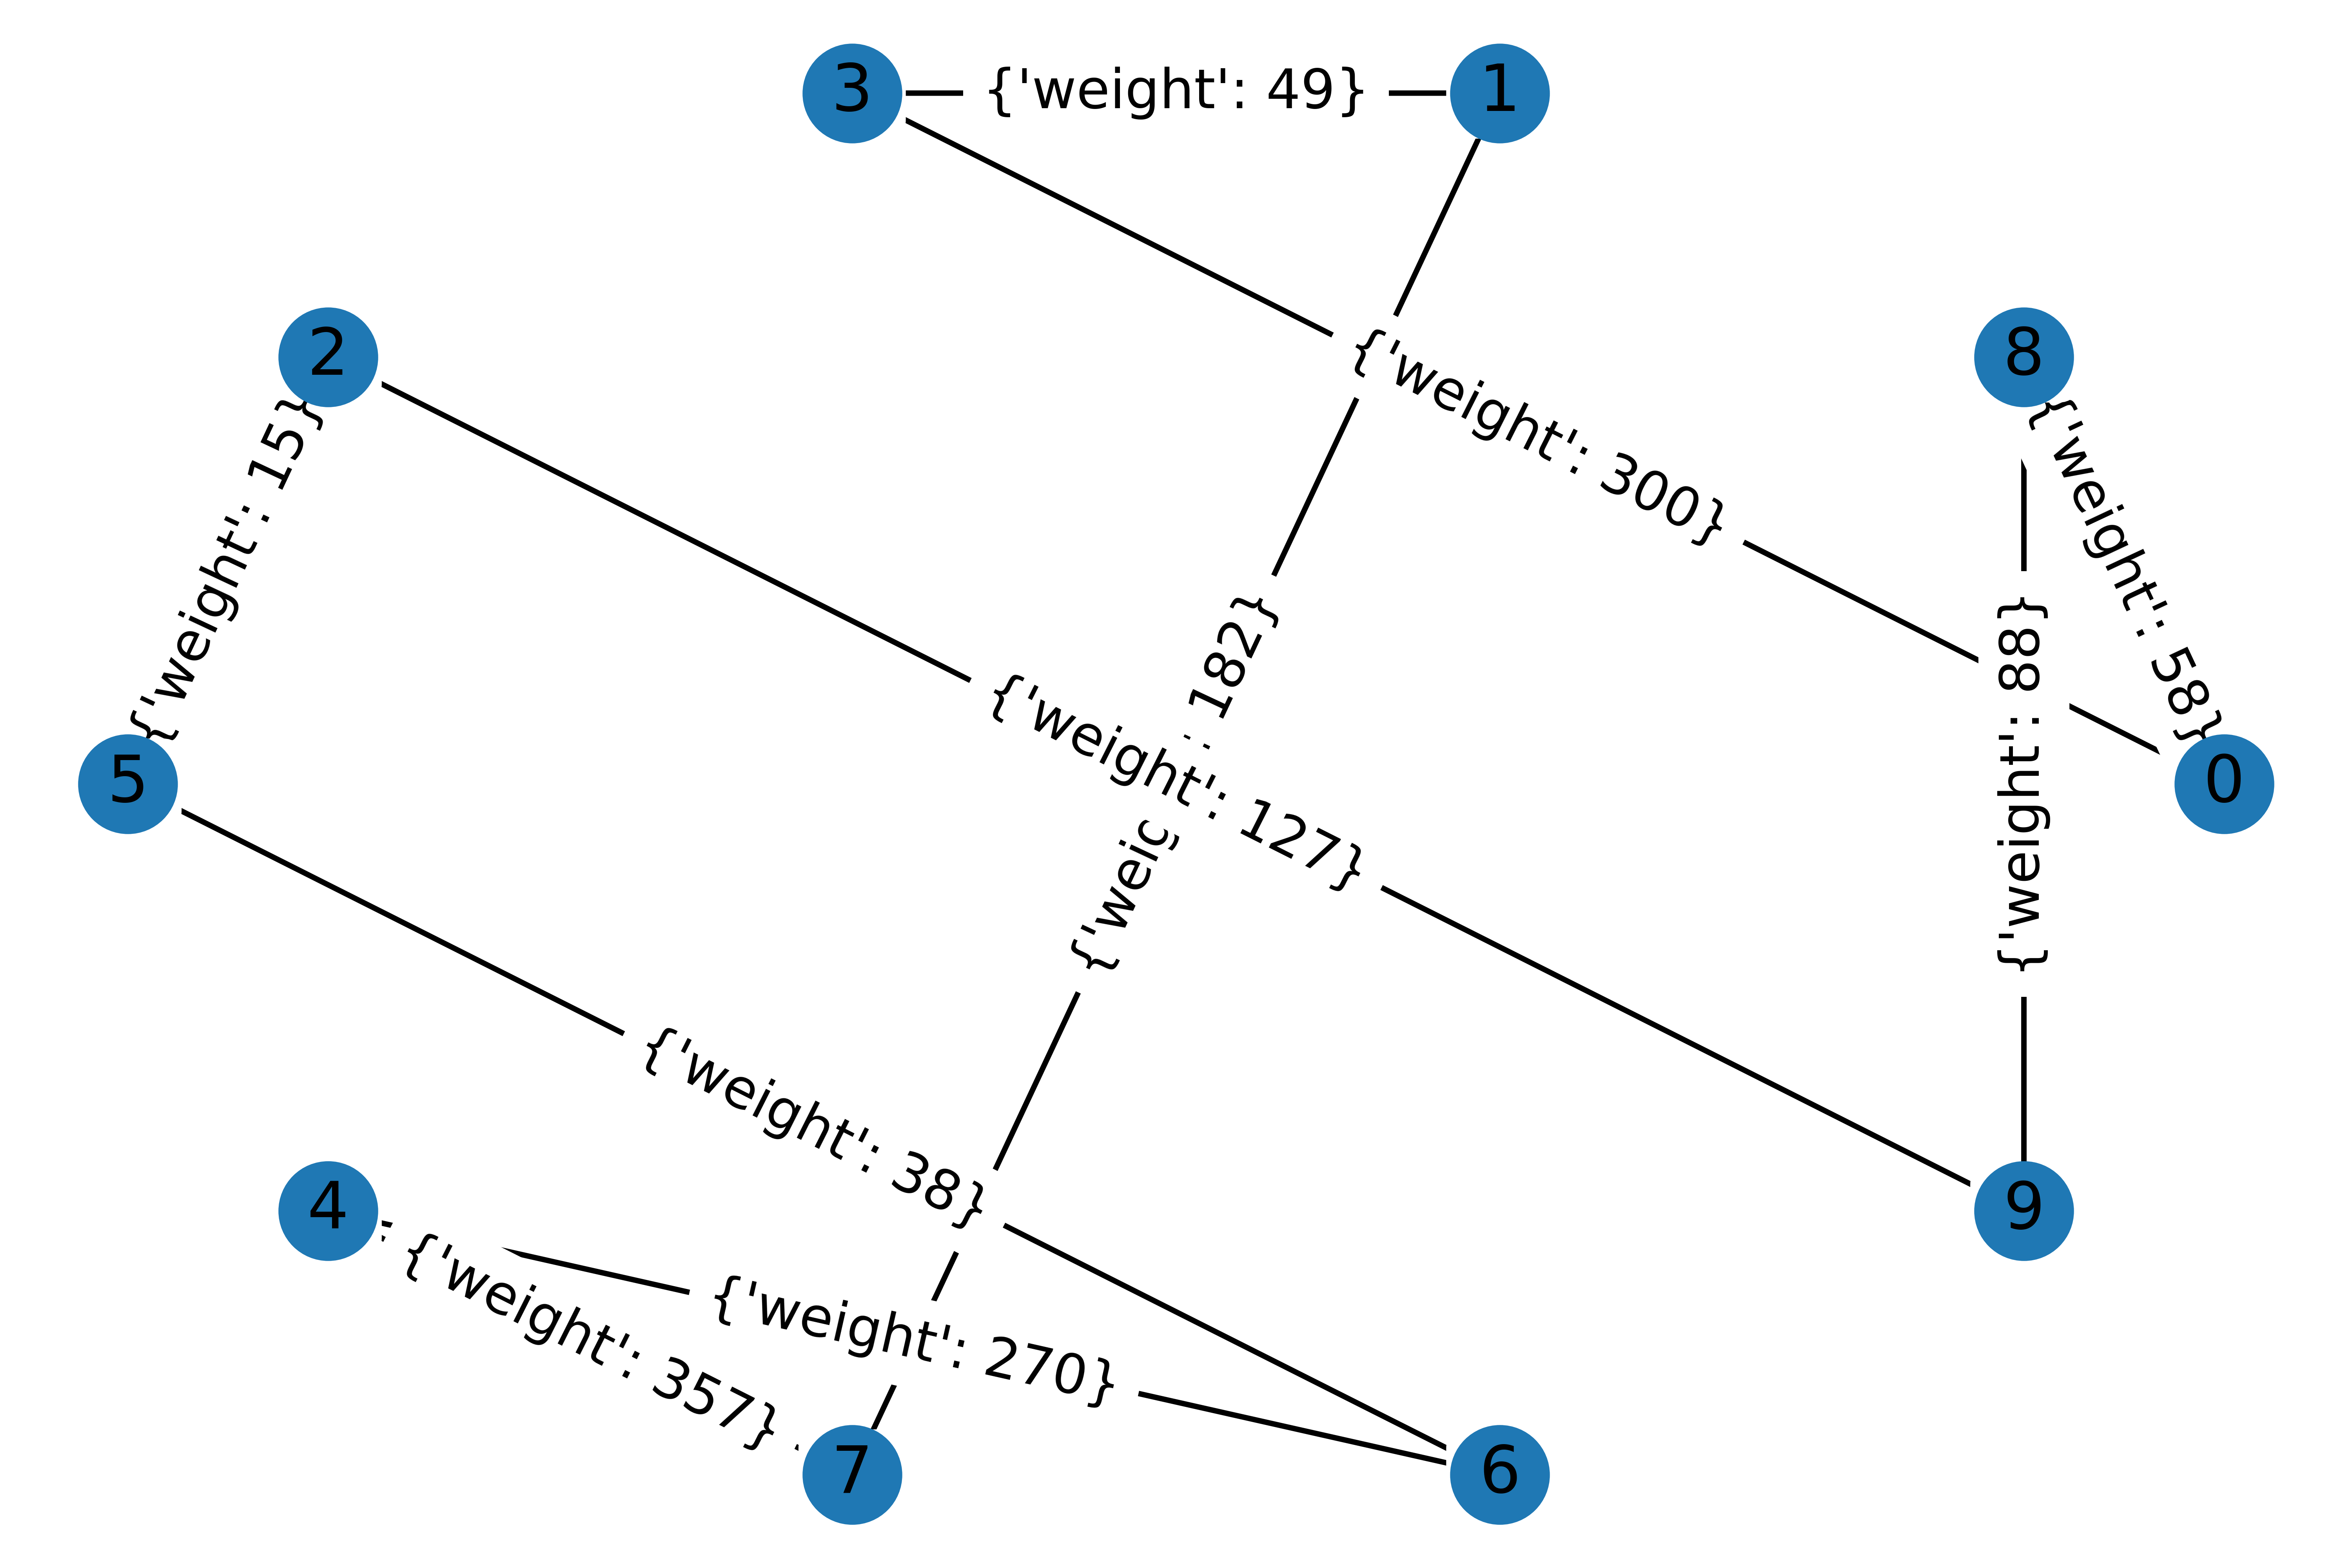
\includegraphics[width=10cm]{primeri/primer2_3opt.png}
 	\caption{3-opt}
	\label{Slika 7}
	\end{figure}
\end{frame}

\begin{frame}
\begin{figure}
  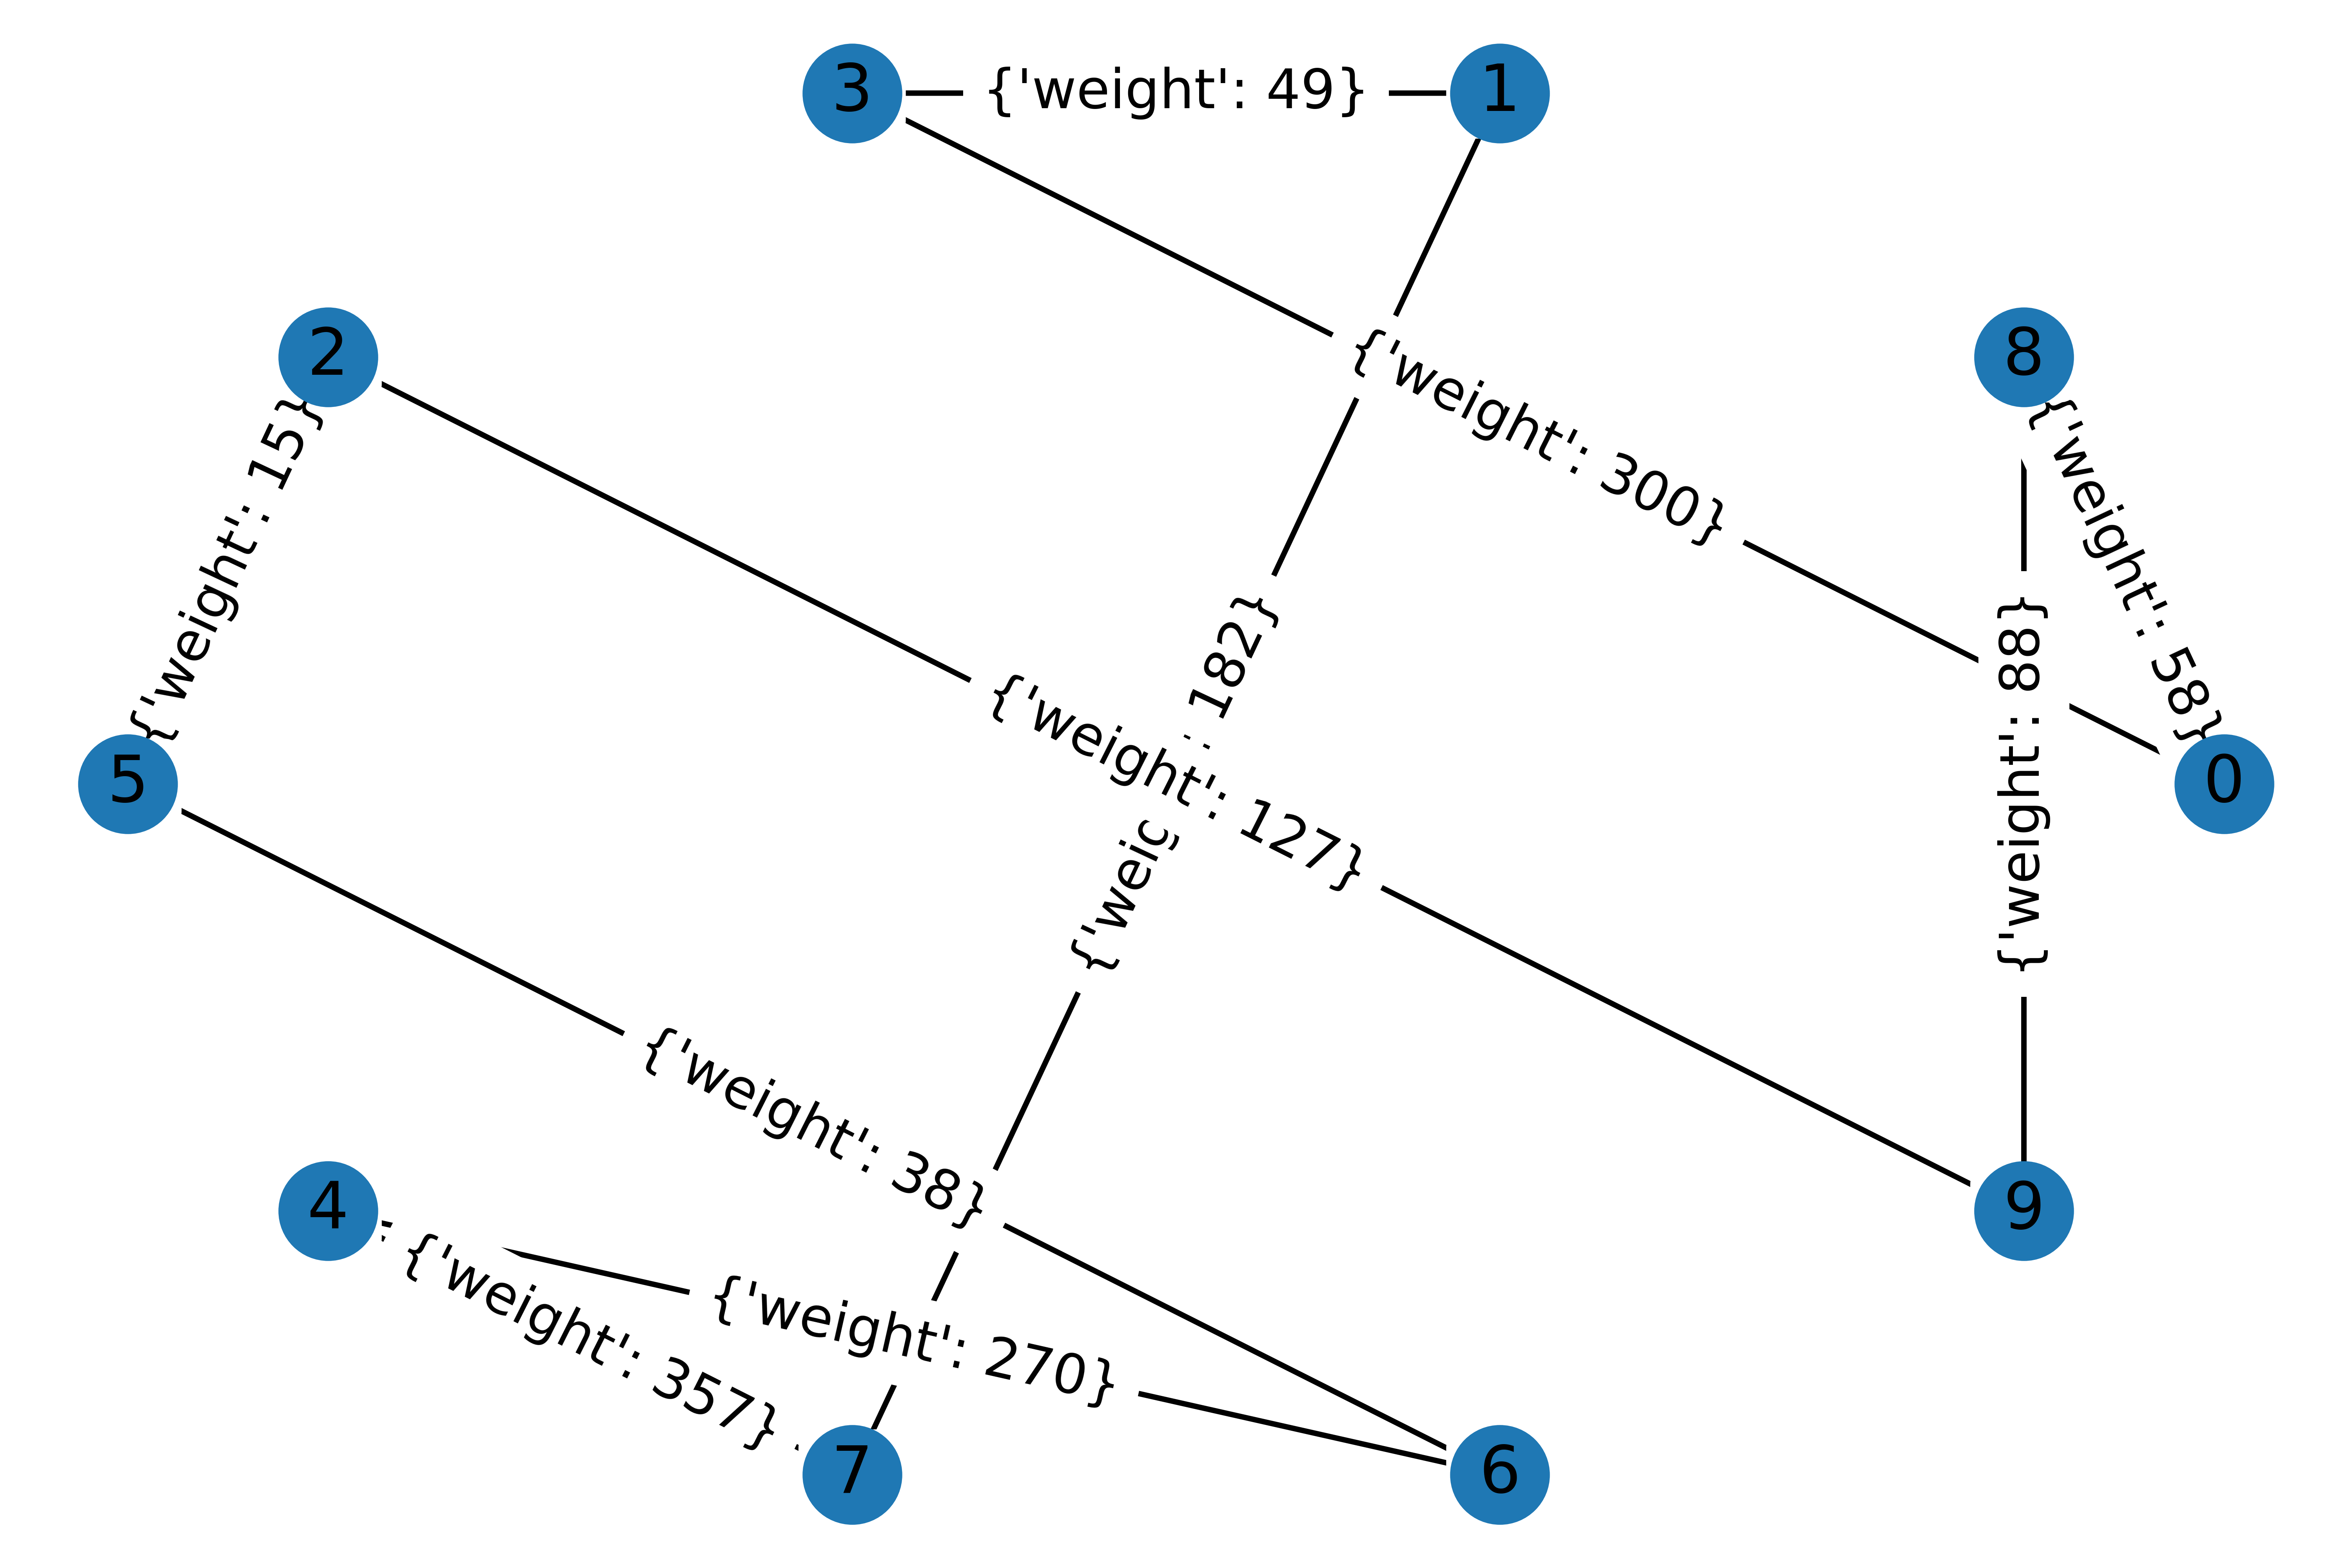
\includegraphics[width=10cm]{primeri/primer2_lk.png}
\caption{LK}
\label{Slika 8}
\end{figure}
\end{frame}

\section[Časovna zahtevnost]{Časovna zahtevnost}
\begin{frame}
\frametitle{Časovna zahtevnost}
\begin{table}[!h]
\begin{tabular}{|c|c|c|c|c|c|c|c|}
\hline
$n$&začetek&2-Opt&cena 2-Opt&3-Opt&cena 3-Opt&LK&cena LK\\\hline
5&49&0,000675&41&0,000276&41&0,000154&41\\\hline
10&4903&0,004748&1595&0,000600&1484&0,000611&1484\\\hline
20&9047&0,03257&1388&0,00801&1555&0,01151&1517\\\hline
30&11825&0,10143&2255&0,01806&1907&0,04639&1729\\\hline
50&23556&0,69378&2833&0,18529&2496&0,30218&2319\\\hline
80&37169&4,97926&3352&0,53484&2890&1,38603&2362\\\hline
100&46984&9,4767&3404&1,97813&2446&2,31723&2235\\\hline
200&98344&194,093&4673&22,9016&3007&13,7700&2832\\\hline
300&156543&1127,92&5365&162,040&2986&94,0348&2630\\\hline
500&244733&7912,40&6689&402,52&3328&496,36&2900\\\hline
\end{tabular}
\caption{Tabela časov izvajanja algoritmov in cen v odvisnosti od $n$}
\label{tabela_casov}
\end{table}
\end{frame}

\begin{frame}
\begin{figure}[!h]
 \begin{center}
  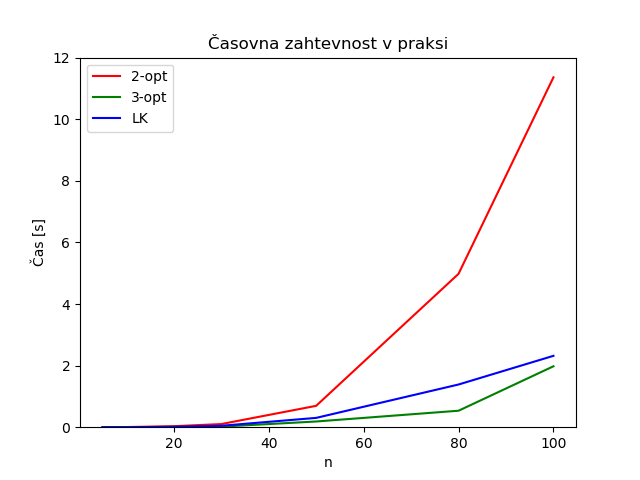
\includegraphics[width=12 cm]{casovna_zahtevnost_do_100.png}
  \caption{Časovna zahtevnost vseh treh algoritmov do $n$ = 100}
  \label{casovna_do_100}
\end{center}
\end{figure}
\end{frame}


\section[Viri]{Viri}
\begin{frame}
\begin{enumerate}

\item A. Hagberg, D. Schult, P. Swart:\emph{NetworkX Refrence, Release 2.4}, [ogled 2.~1.~2020], dostopno na \url{https://networkx.github.io/documentation/stable/_downloads/networkx_reference.pdf}

\item \emph{Optimization with 2-OPT - Part 1}, [ogled 3.~1.~2020], dostopno na \url{http://pedrohfsd.com/2017/08/09/2opt-part1.html}

\item \emph{2-opt}, [ogled 3.~1.~2020], dostopno na \url{https://en.wikipedia.org/wiki/2-opt}

\item \emph{3-opt}, [ogled 4.~1.~2020], dostopno na \url{https://en.wikipedia.org/wiki/3-opt}

\item \emph{3-opt: basic algorithm}, [ogled 4.~1.~2020], dostopno na \url{https://tsp-basics.blogspot.com/2017/03/3-opt-iterative-basic-algorithm.html}

\item D. Karapetyan, G. Gutin, \emph{Lin-Kernighan Heuristic Adaptations for the Generalized Traveling Salesman Problem}, [ogled  8.~1.~2020], dostopno na \url{https://arxiv.org/pdf/1003.5330.pdf}
\end{enumerate}
\end{frame}

\end{document}